%%%%%%%%%%%%%%%%%%%%%%%%%%%%%%%%%%%%%%%%%
% Dreuw & Deselaer's Poster
% LaTeX Template
% Version 1.0 (11/04/13)
%
% Created by:
% Philippe Dreuw and Thomas Deselaers
% http://www-i6.informatik.rwth-aachen.de/~dreuw/latexbeamerposter.php
%
% This template has been downloaded from:
% http://www.LaTeXTemplates.com
%
% Edited by: Manfred Brill
%
% License:
% CC BY-NC-SA 3.0 (http://creativecommons.org/licenses/by-nc-sa/3.0/)
%%%%%%%%%%%%%%%%%%%%%%%%%%%%%%%%%%%%%%%%%

% ----------------------------------------------------------------------------------------
%  Kopf- und Fusszeile werden in beamertheme16pd2.sty definiert!
% ----------------------------------------------------------------------------------------

%----------------------------------------------------------------------------------------
%   PACKAGES AND OTHER DOCUMENT CONFIGURATIONS
%----------------------------------------------------------------------------------------
\documentclass[final,hyperref={pdfpagelabels=false}]{beamer}

\usepackage{wrapfig}
\usepackage[orientation=portrait, size=a0, scale=1.2]{beamerposter}
\usetheme{I6pd2} % sty-file, verändert mit HS Logo und Box für Titel

\usepackage[german]{babel}
%\usepackage[english]{babel} % English language/hyphenation
\usepackage{amsmath,amsthm,amssymb,latexsym}

%\usepackage{times}\usefonttheme{professionalfonts}  % Uncomment to use Times as the main font
%\usefonttheme[onlymath]{serif} % Uncomment to use a Serif font within math environments

\boldmath % Use bold for everything within the math environment

\usepackage{booktabs} % Top and bottom rules for tables
\usepackage{multicol}
\usepackage{caption}
\usepackage{subcaption}
\usepackage{hyperref}
\usepackage[misc]{ifsym}
\usepackage[export]{adjustbox}
\usepackage{fontawesome}

\graphicspath{{figures/}} % Location of the graphics files

\usecaptiontemplate{\small\structure{\insertcaptionname~\insertcaptionnumber: }\insertcaption}
 % A fix for figure numbering

%----------------------------------------------------------------------------------------
%  Titel
\title{\huge Visual$\:$Raytrace: An Immersive Learning Application}
\author{Manfred Brill, Benedict S\"arota}
\institute{Department of Computer Science and Microsystems Technology\\University of Applied Sciences Kaiserslautern}
%----------------------------------------------------------------------------------------

\begin{document}

\addtobeamertemplate{block end}{}{\vspace*{1ex}} % White space under blocks

\begin{frame}[t] % The whole poster is enclosed in one beamer frame

\vspace*{0.75cm}

\begin{columns}[t] % Spalten für den ersten Teil
\begin{column}{.025\textwidth}\end{column} % Empty spacer column

\begin{column}{.465\textwidth} % Das erste mit einem Raytracer gerenderte Bild
\begin{block}{Whitted Raytracing}
    \begin{figure}
    	\centering
        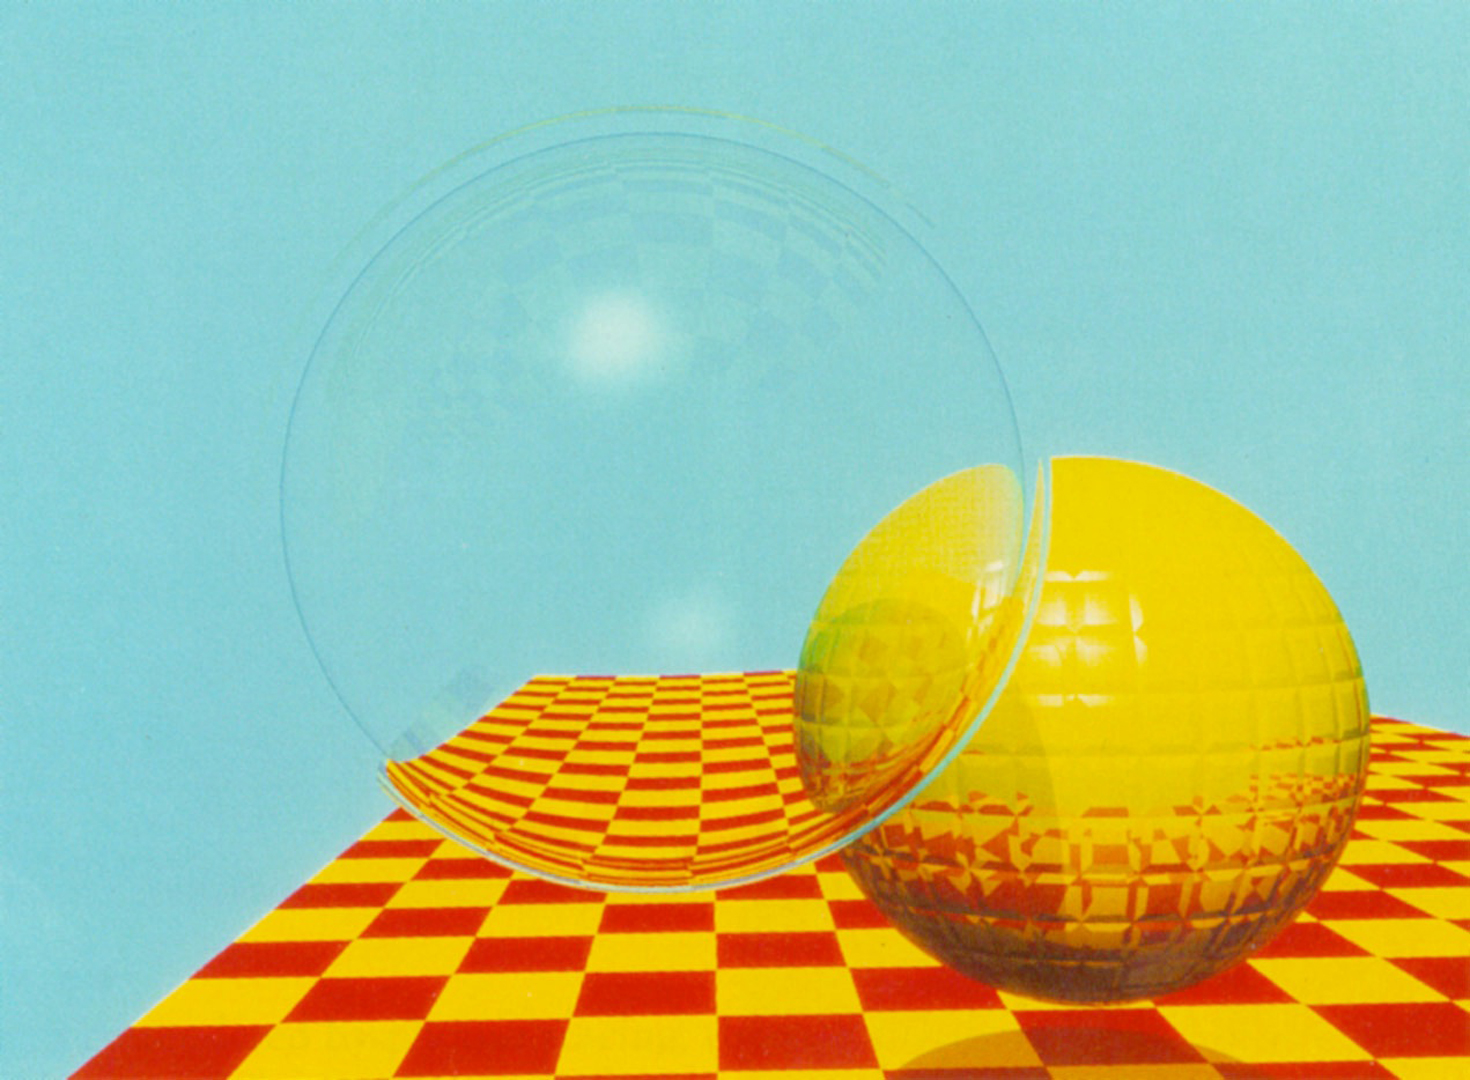
\includegraphics[width=0.65\linewidth]{whitted02}
    \end{figure}
\end{block}

\vspace*{2.0cm}

\begin{block}{A Raytracer in a Virtual Environment}
    \begin{figure}
    	\centering
        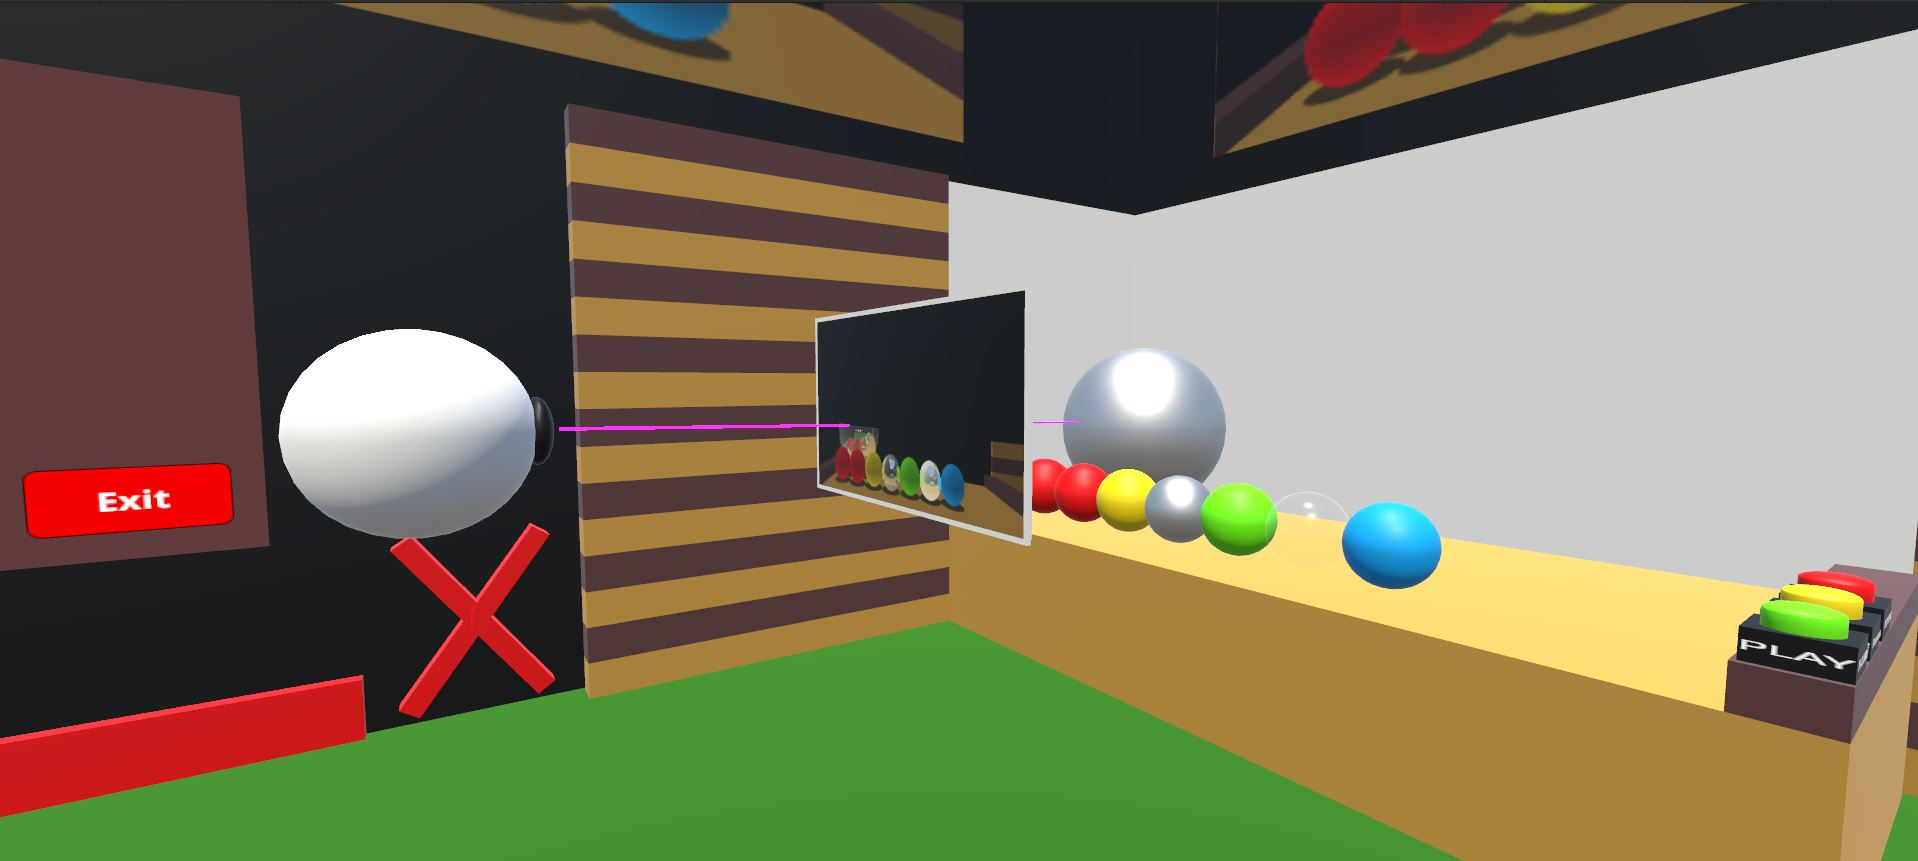
\includegraphics[width=0.95\linewidth]{duringProcess}
    \end{figure}
\end{block}

\begin{block}{Ray-Sphere Intersection}
    \begin{figure}
    	\centering
        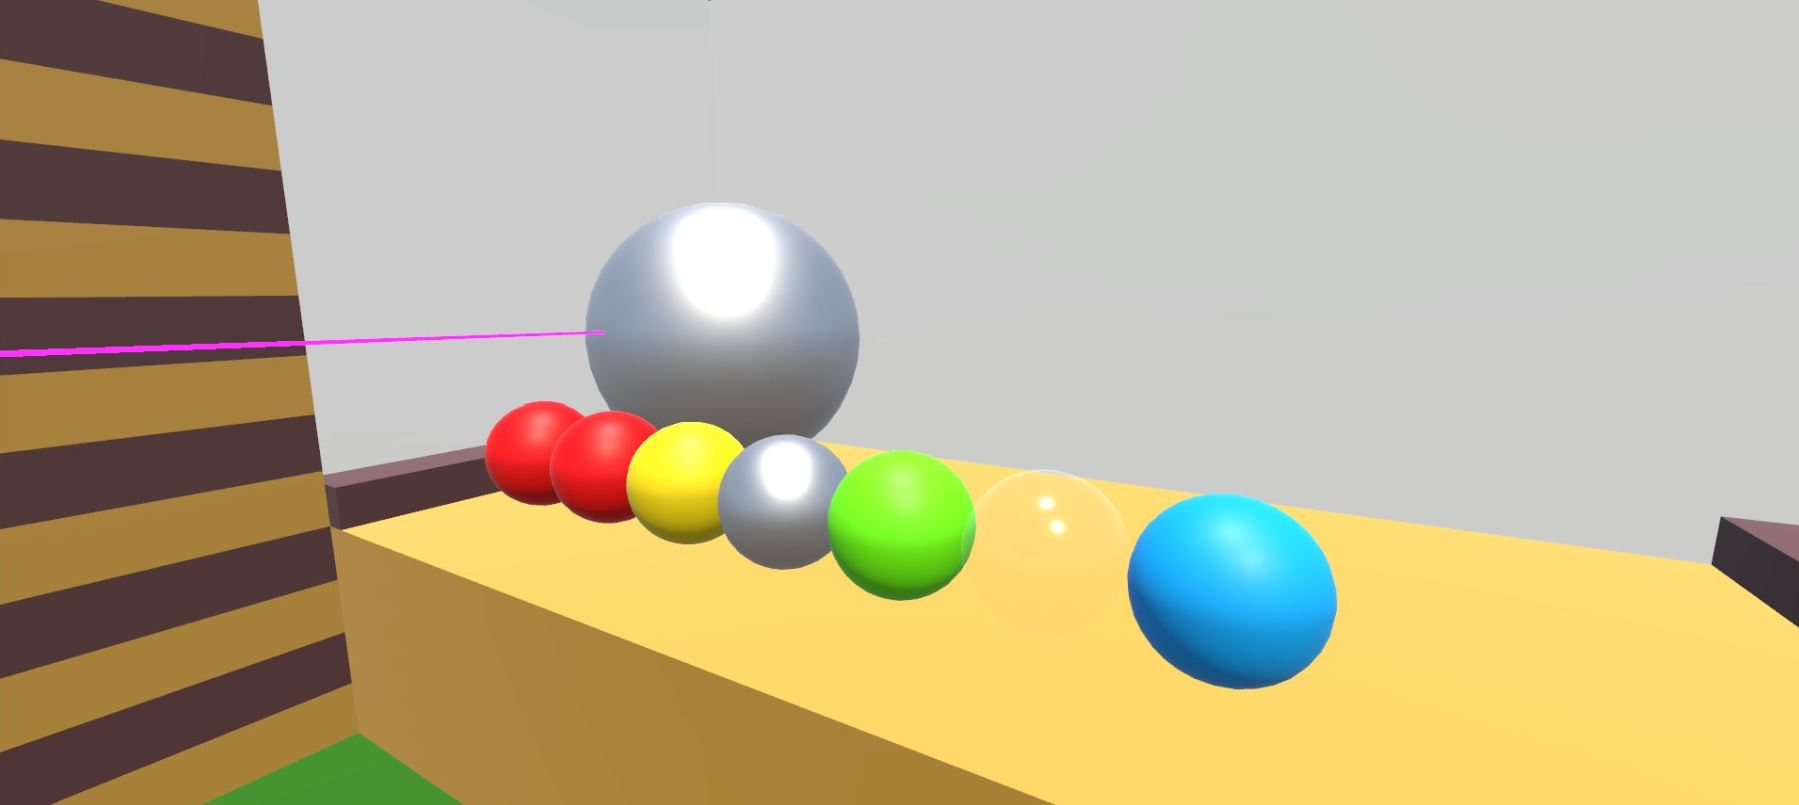
\includegraphics[width=0.95\linewidth]{duringProcessHitObjects}
    \end{figure}
\end{block}

\begin{block}{Interactive Scene Definition}
    \begin{figure}
    	\centering
        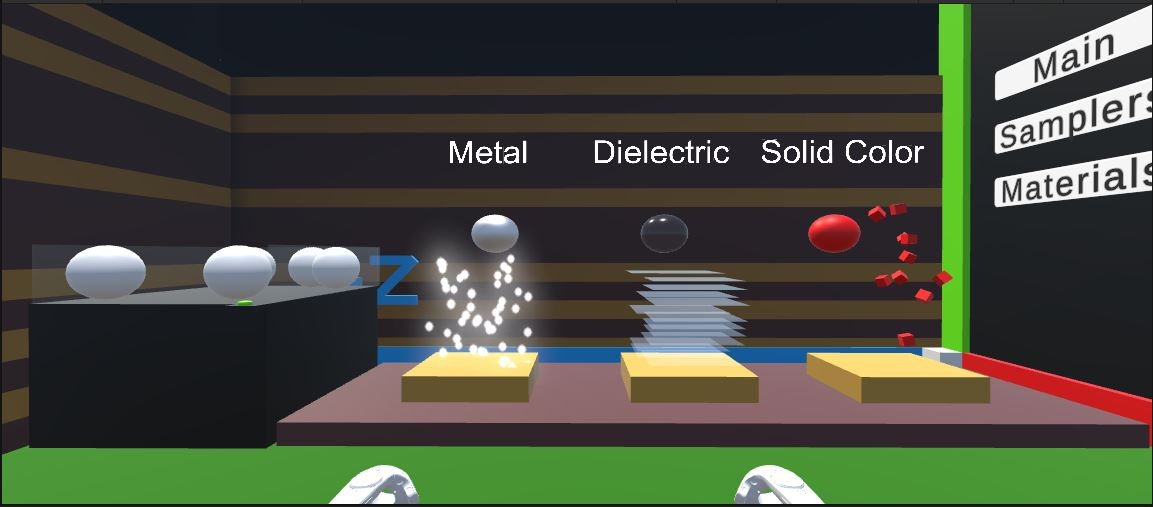
\includegraphics[width=0.95\linewidth]{sphereCreating}
    \end{figure}
\end{block}

\end{column}

\begin{column}{.025\textwidth}\end{column} % Empty spacer column

\begin{column}{0.465\textwidth} % Text zu immersive learning
\begin{block}{Immersive Learning}
    \vspace{2.2cm}

   \begin{itemize}
   \item Raytracing is one of the major topics in computer graphics classes.
   \item Students have to implement their own version of a working raytracer.
   \item To implement a raytracer students need to understand the basic concepts of computer graphics
   like coordinate systems, camera, lighting or reflection.
   \item Key for the successful implementation of a raytracer by the students: develop a high spatial imagination.
   \item The immersive learning application \textbf{Visual Raytrace} supports the transfer from 3D space
   to a programming language and deepens the understanding of the basic concepts of a raytracer.

       \vspace{1.55cm}$\:$
   \end{itemize}

\end{block}

\vspace*{2.0cm}

\begin{block}{Unity and C\#}
    \begin{figure}
    	\centering
        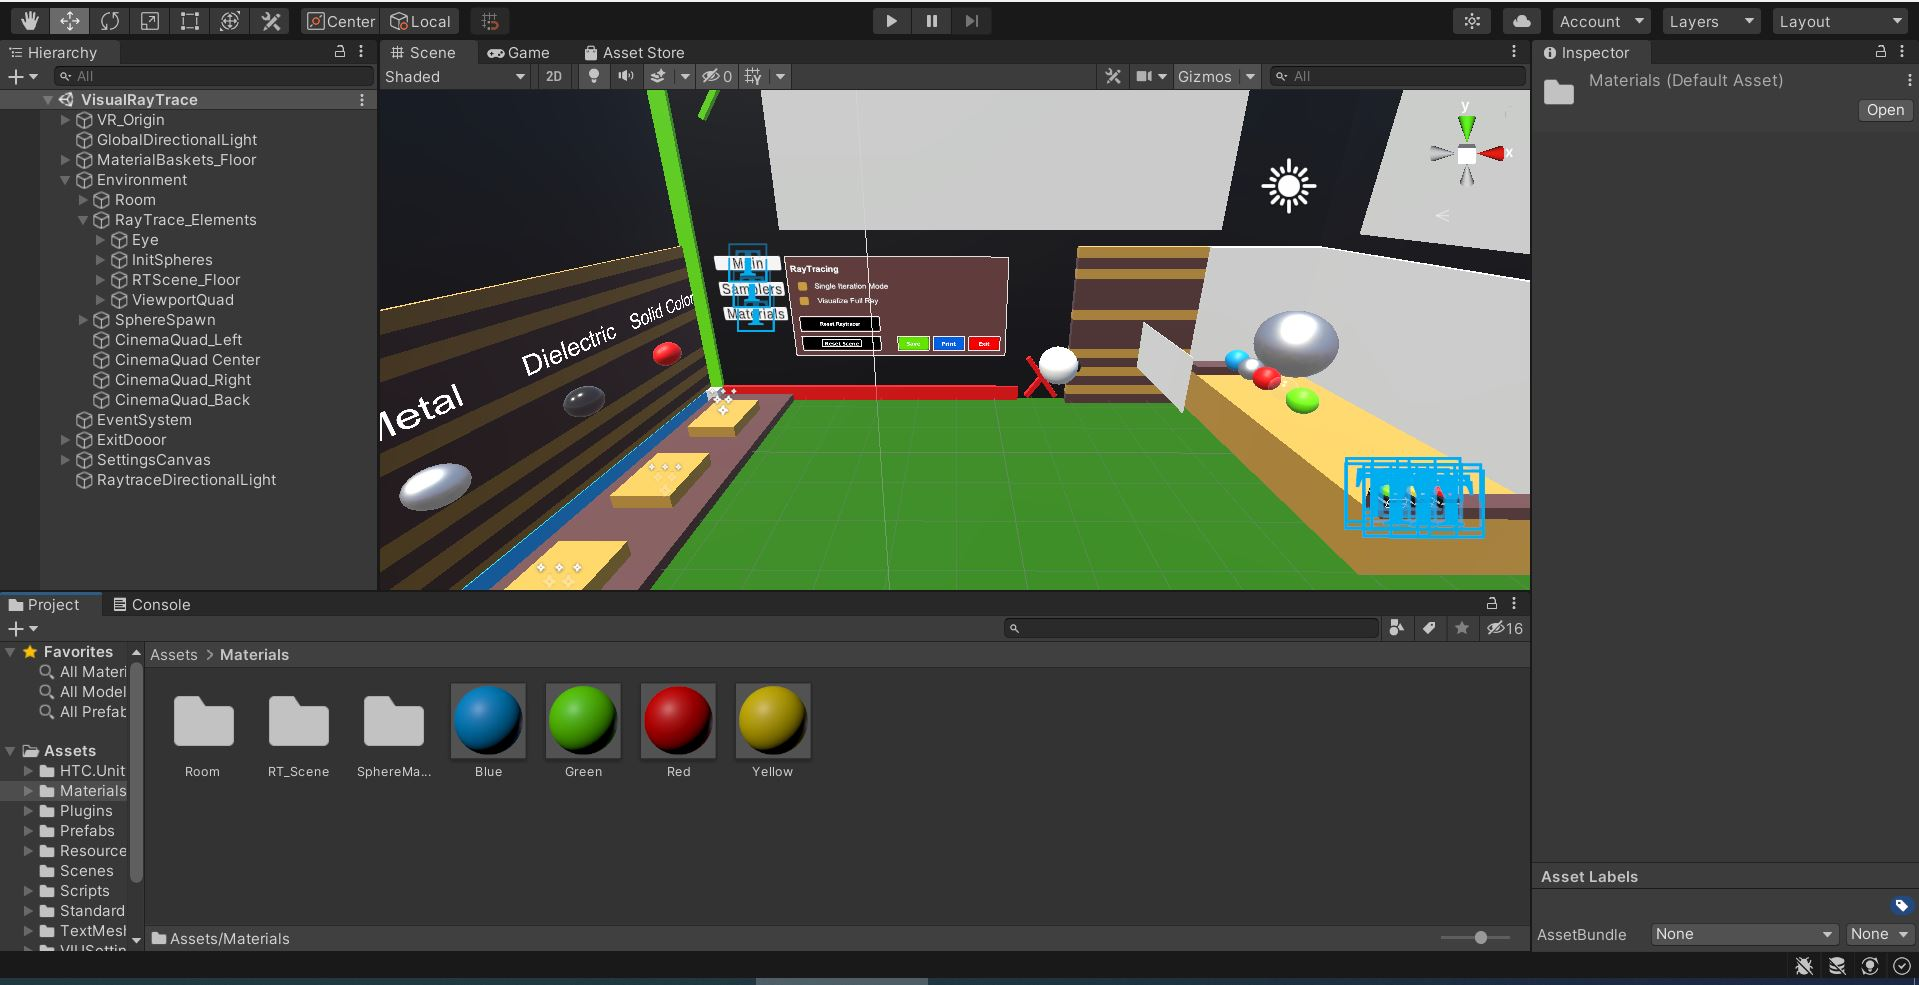
\includegraphics[width=0.95\linewidth]{unityIDE}
    \end{figure}
\end{block}

\begin{block}{A Virtual Framebuffer and a Virtual Ray}
    \begin{figure}
    	\centering
        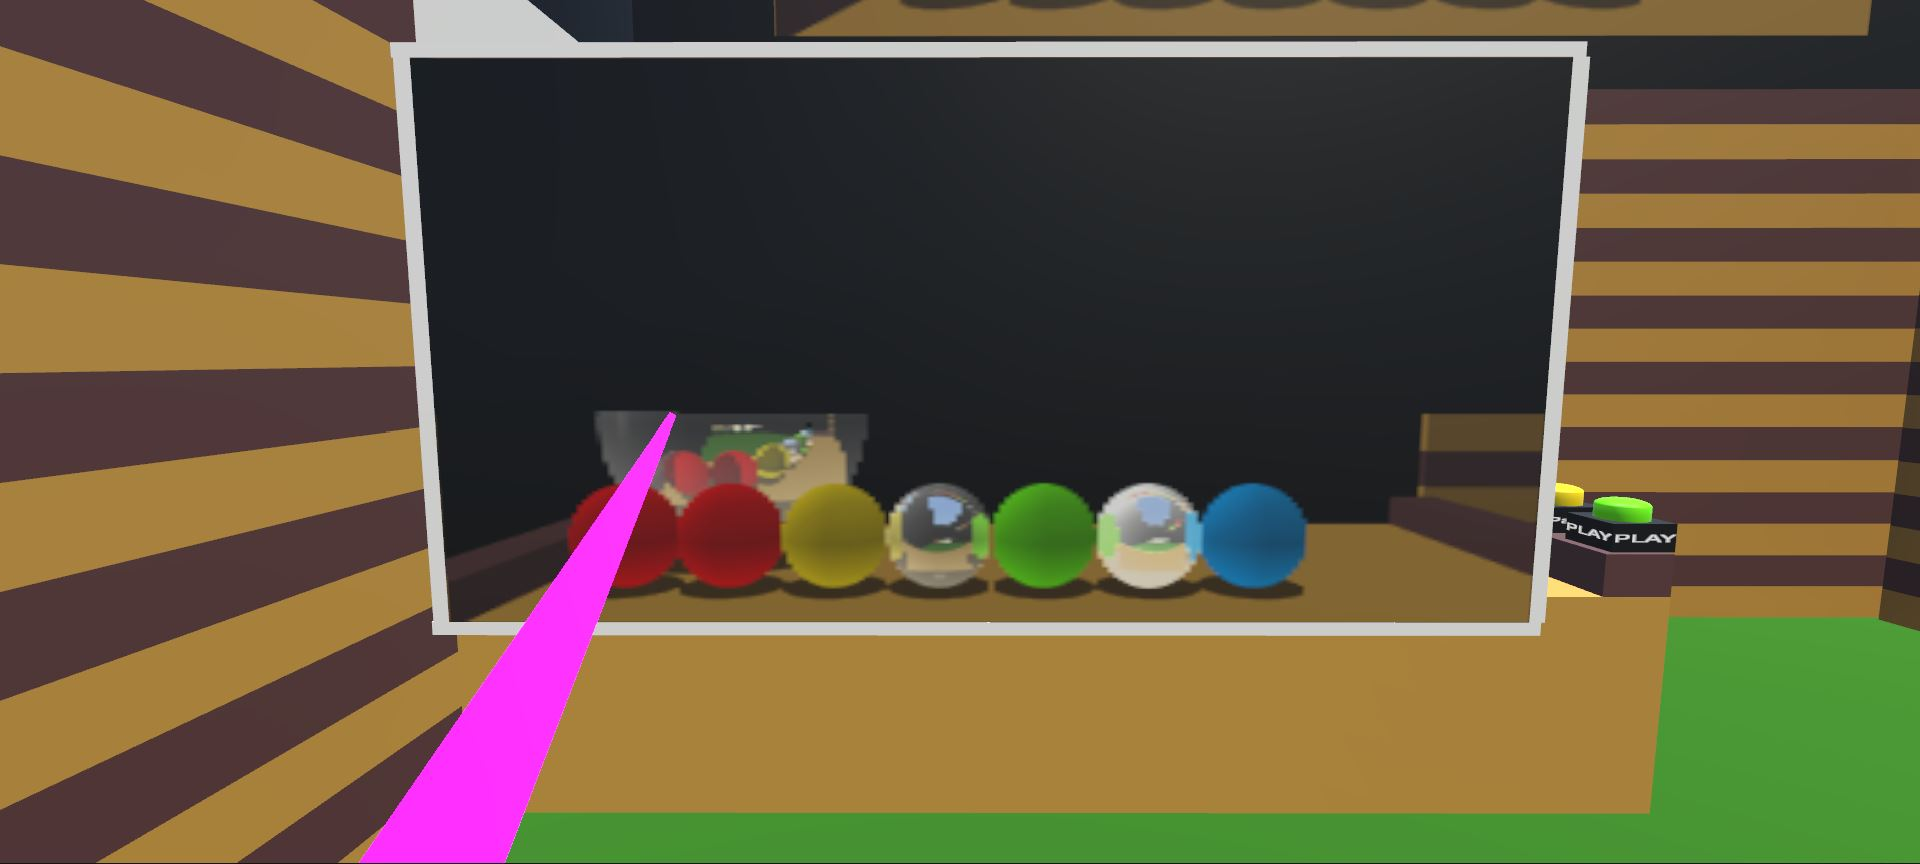
\includegraphics[width=0.95\linewidth]{duringProcessEyeView}
    \end{figure}
\end{block}

\begin{block}{Settings for the Raytracer}
    \begin{figure}
    	\centering
        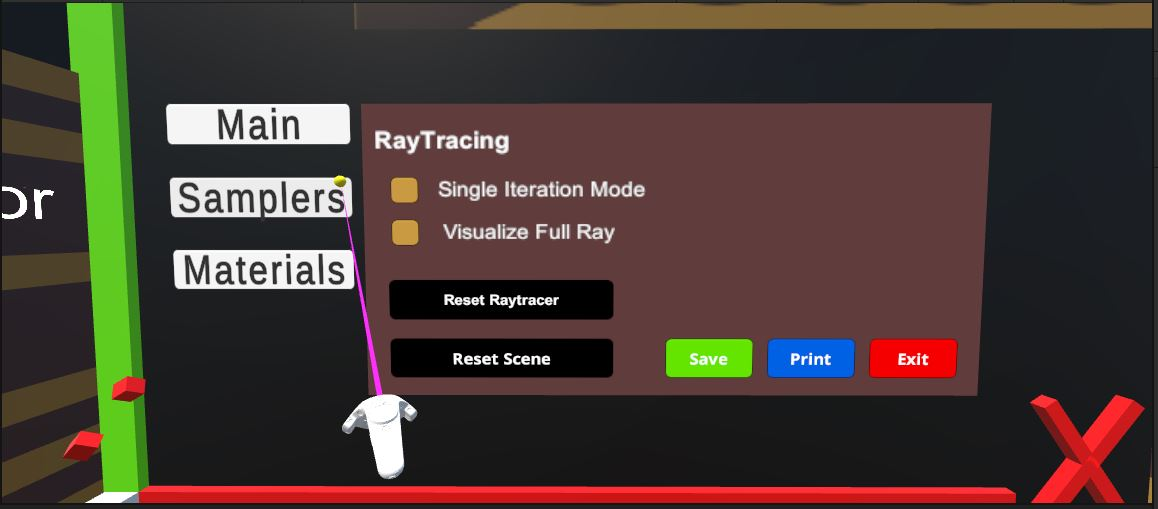
\includegraphics[width=0.95\linewidth]{settings}
    \end{figure}
\end{block}
\end{column}
\begin{column}{.025\textwidth}\end{column} % Empty spacer column
\end{columns}

\vspace*{1.25cm}

% QR-Code, Literaturverzeichnis
\begin{columns}[t]

\vspace*{0.2cm}

\begin{column}{0.15\textwidth}

\begin{figure}[h]

\vspace*{1.0cm}

\centering
\includegraphics[scale=1.25]{qrCode}
\end{figure}
\end{column}

\begin{column}{0.025\textwidth}\end{column} % Empty spacer column

\begin{column}{0.3\textwidth}
\vspace*{3.0cm}
\begin{itemize}
\item[] \Letter\ \href{benedict.saerota@hs-kl.de}{benedict.saerota@hs-kl.de}
\item[] \Letter\ \href{manfred.brill@hs-kl.de}{manfred.brill@hs-kl.de}
\item[]
\item[] \includegraphics[scale=0.75]{icon/githubIcon} \href{https://github.com/VRLAB-HSKL/RayTracing}{http://github.com/VRLAB-HSKL/RayTracing}
\end{itemize}
\end{column}

\begin{column}{0.025\textwidth}\end{column} % Empty spacer column

\begin{column}{0.465\textwidth}
\nocite{*} % Alles zitieren in sample.bib
\begin{block}{References}
 \bibliographystyle{eg-alpha}
 \bibliography{sample}
\end{block}
\end{column}

\begin{column}{0.025\textwidth}\end{column} % Empty spacer column

\end{columns}

\end{frame} % Ende des frames, der das Poster enthält
\end{document} 